\subsection{Hessian profiling}
\label{sec:hessianprofiling}

% Results of the Hessian profiling using HERAPDF2.0 as input.


Similarly to the reweighting method, that was used to estimate the effect of including Lattice
data to the Monte Carlo PDFs (NNPDF3.0) in Sec.\ref{}, in case of Hessian PDF sets a profiling
method~\cite{Paukkunen:2014zia,Camarda:2015zba} can be used.
In the following we have used the same Lattice data on moments to estimate the impact
on a HERAPDF20 unpolarized Hessian PDFs~\cite{Abramowicz:2015mha}. We choose HERAPDFs as a
representative set of Hessian PDFs. It has an additional advantage of using $\Delta\chi^2=1$ for
defining Hessian error PDFs which ensures a one to one correspondence of the profiling and
reweighting methods.
We have performed the study assuming the same 3 scenarios for the errors of the Lattice data,
see Table~\ref{tab:scenarios}. The study was performed using the xFitter program~\cite{Alekhin:2014irh}.

The central values of the considered moments are obtained using the central PDFs and the corresponding
errors are calculated in the following way:
\begin{equation}
\delta\mathcal{F}_i = \frac{1}{2} \sqrt{\sum_{k}\left(\mathcal{F}_i(f_k^+)-\mathcal{F}_i(f_k^-)\right)^2},
\quad i=1,\ldots,N_{\rm mom}
\end{equation}
where $k$ numbers the error PDFs.

The results of the profiling are shown in Table~\ref{tab:unpolmomentsProf} where the uncertainties
of the considered moments are displayed in case of initial HERAPDF20 and after including the Lattice
moments data in the three scenarios.
%%%%%%%%%%%%%%%%%%%%%%%%%%%%%%%%%%%%%%%%%%%%%%%%%%%%%%%%
\begin{table}[h]
  \centering
  \renewcommand{\arraystretch}{1.3} 
\begin{tabular}{c||c|c|c|c}
  \hline &  Original  & Scen A  &  Scen B  &  Scen C  \\
  \hline
  \hline
  $\la x\ra_{u^+}$     &  $0.3720\pm 0.0036$  &  $0.3720\pm 0.0030$  &  $0.3720\pm 0.0027$  &  $0.3720\pm 0.0020$ \\
  $\la x\ra_{d^+}$     &  $0.1845\pm 0.0053$  &  $0.1845\pm 0.0028$  &  $0.1845\pm 0.0023$  &  $0.1845\pm 0.0015$ \\
  $\la x\ra_{s^+}$     &  $0.0346\pm 0.0037$  &  $0.0346\pm 0.0015$  &  $0.0346\pm 0.0012$  &  $0.0346\pm 0.0009$ \\
  $\la x\ra_{g}$       &  $0.4006\pm 0.0078$  &  $0.4006\pm 0.0042$  &  $0.4006\pm 0.0035$  &  $0.4006\pm 0.0024$ \\
  $\la x\ra_{u^+-d^+}$ &  $0.1875\pm 0.0074$  &  $0.1875\pm 0.0045$  &  $0.1875\pm 0.0039$  &  $0.1875\pm 0.0027$ \\
  \hline
\end{tabular}
\caption{\small Values of the unpolarized PDF moments
  used as pseudo-data, as well as the corresponding results
  after the profiling has been performed for the
three scenarios summarized in Table~\ref{tab:scenarios}.
%
The HERAPDF20 PDFs were used, the PDF uncertainties quoted correspond in all cases to 68\%
CL intervals.
\label{tab:unpolmomentsProf}
}
\end{table}
%%%%%%%%%%%%%%%%%%%%%%%%%%%%%%%%%%%%%%%%%%%%%%%%%%%%%%%%
%
Additionally, in Fig.~\ref{fig:pdfsProf}, we show the impact of the Lattice data on the PDFs by
comparing the relative errors of the PDFs in scenarios A, B and C with initial HERAPDF20 errors.
%
%------------------------------------------------------
\begin{figure}[!t]
\centering
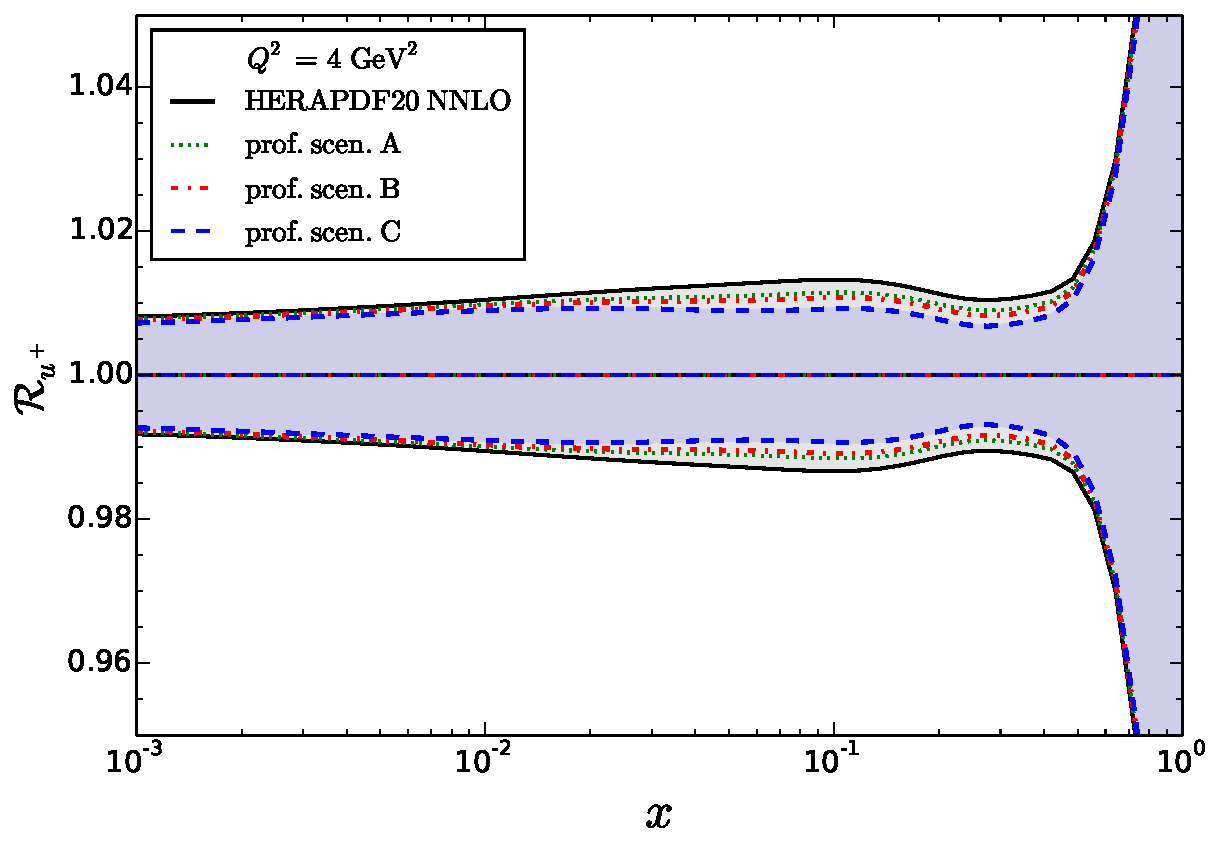
\includegraphics[width=0.3\textwidth]{plots/ratio_uPubar_Q2.pdf}
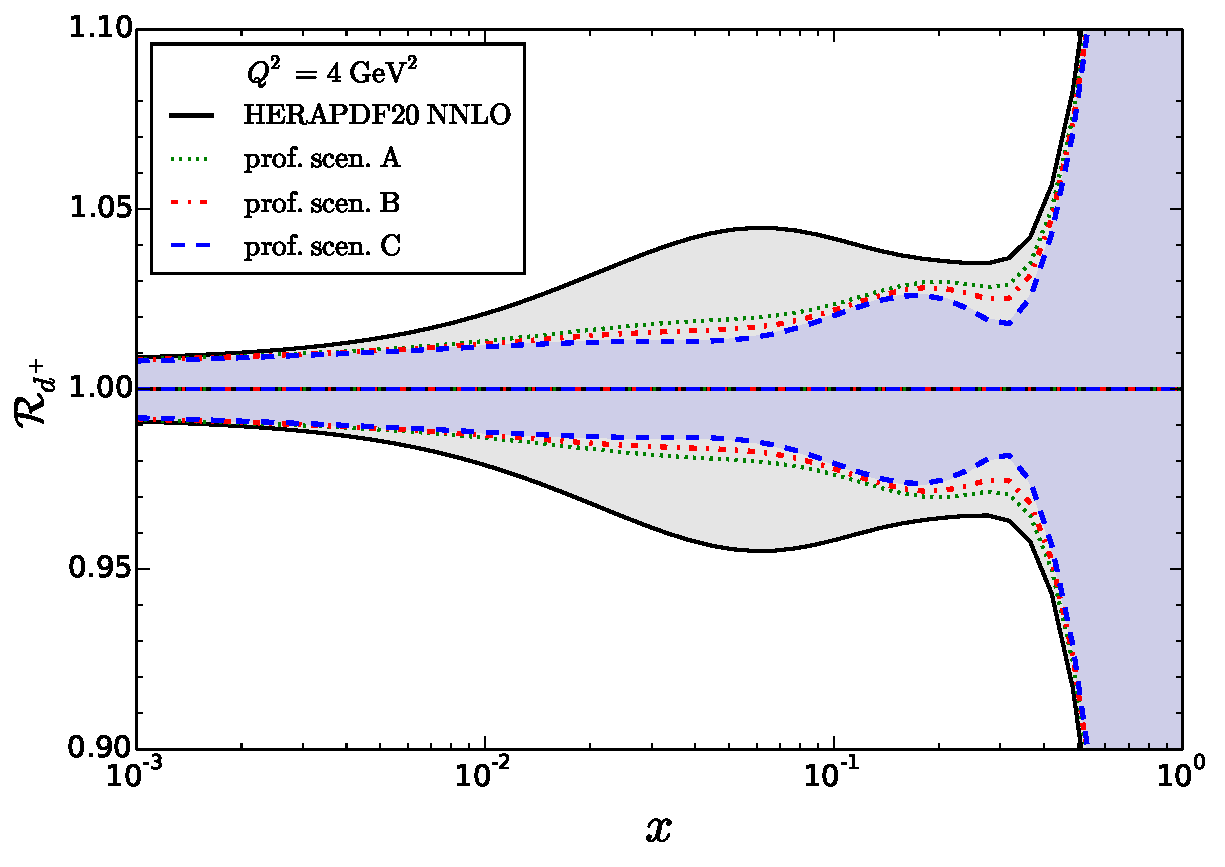
\includegraphics[width=0.3\textwidth]{plots/ratio_dPdbar_Q2.pdf}
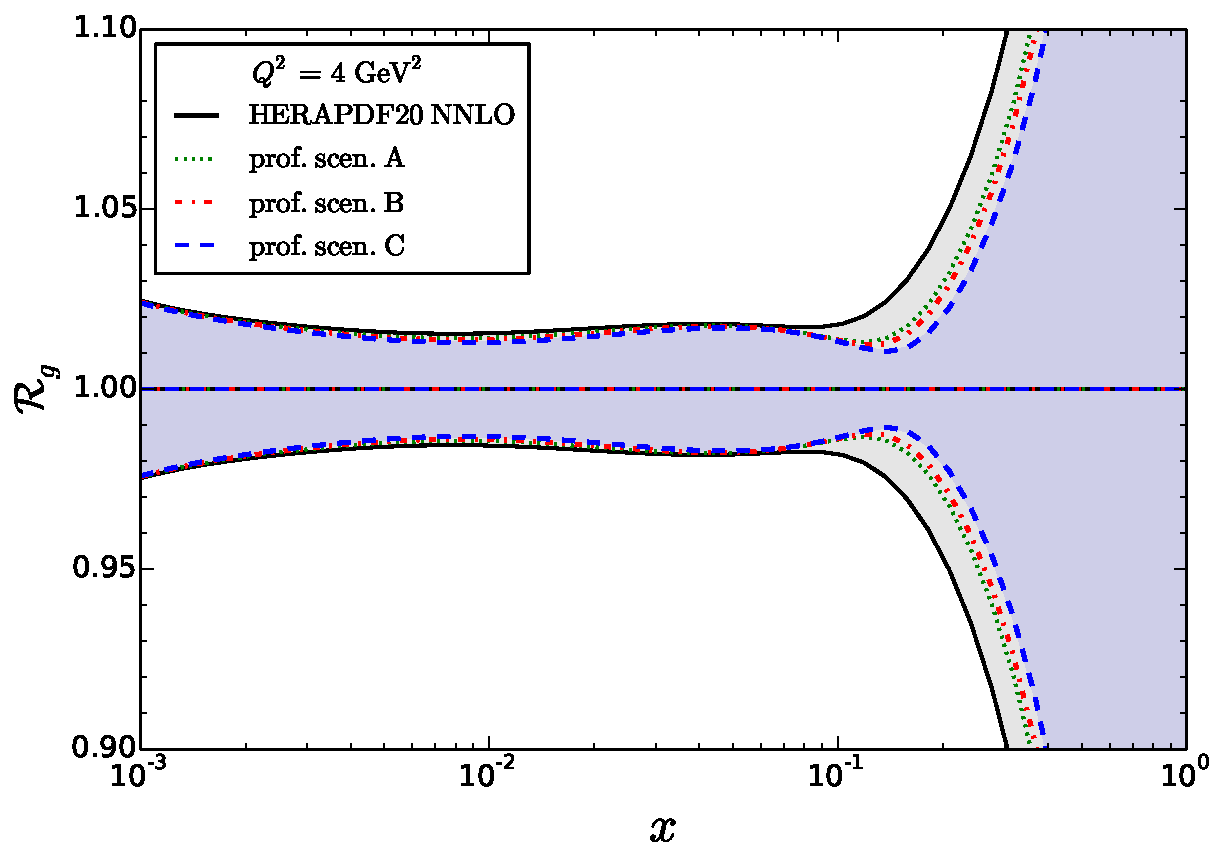
\includegraphics[width=0.3\textwidth]{plots/ratio_g_Q2.pdf}
\\
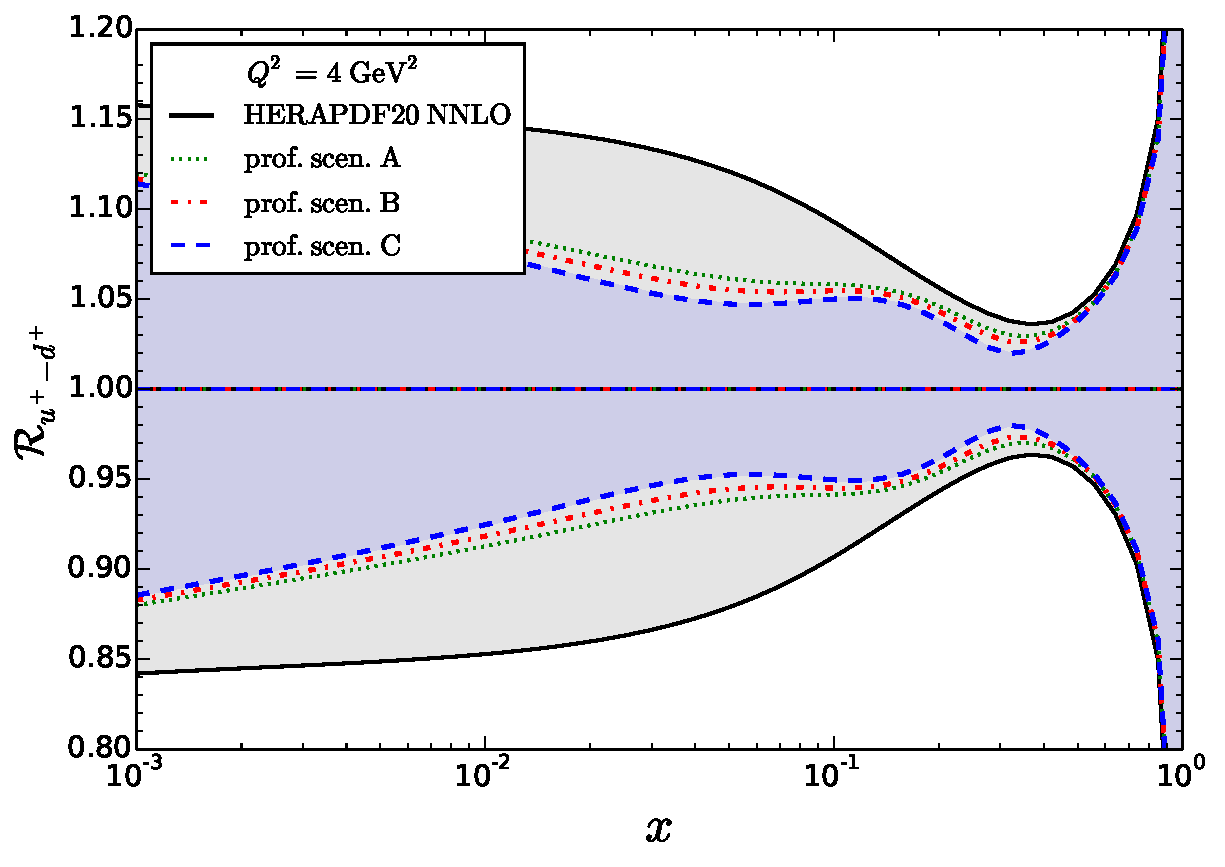
\includegraphics[width=0.3\textwidth]{plots/ratio_uPubarMdMdbar_Q2.pdf}
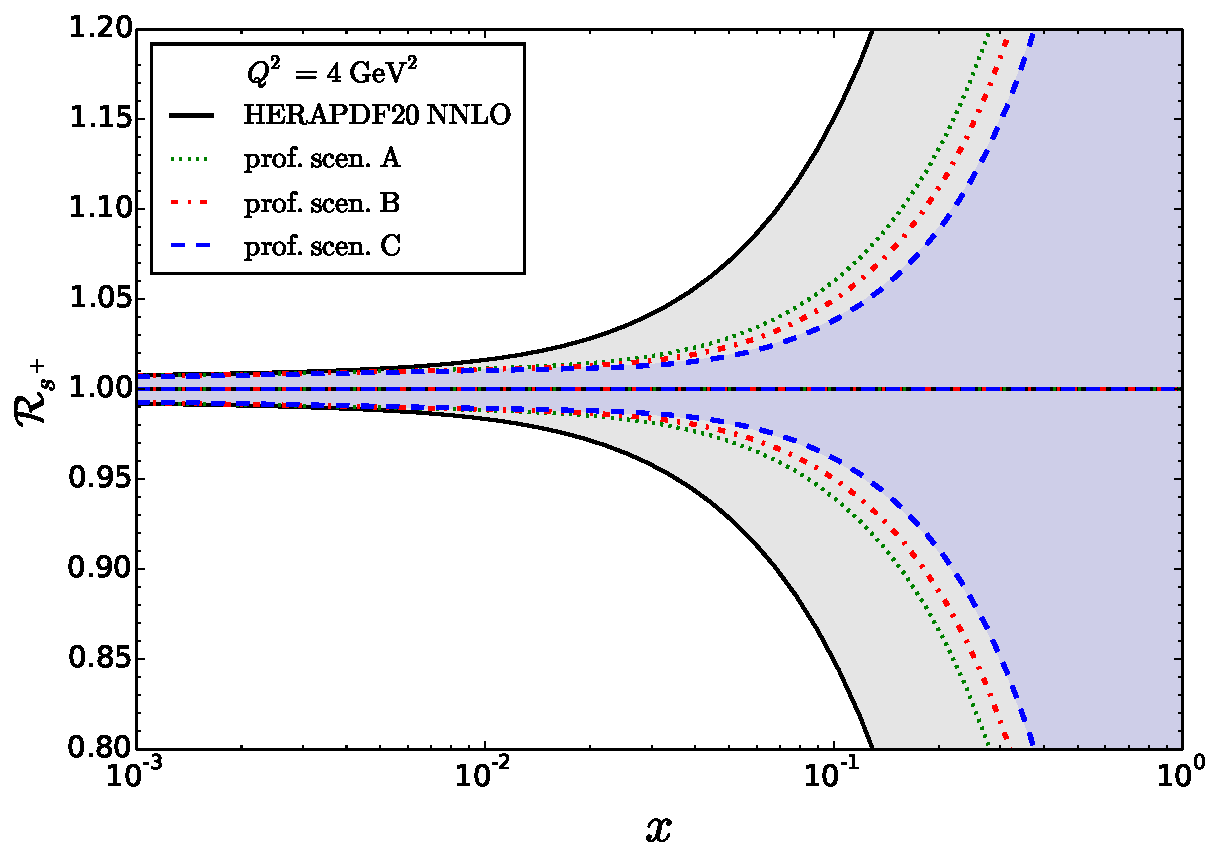
\includegraphics[width=0.3\textwidth]{plots/ratio_sPsbar_Q2.pdf}
\caption{\small Combinations of PDFs: $u^+$, $d^+$, $g$, $u^+-d^+$, $s^+$ at scale $Q^2=4$ GeV$^2$
for initial HERAPDF20 compared with the PDFs resulting from including Lattice moments
data in scenarios A, B and C.
}
\label{fig:pdfsProf}
\end{figure}
%----------------------------------------------------------
%
%
\vspace{1cm}
\\
==============================================\\
==============================================\\
A few sentences about profiling -- that should probably go to the beginning of Sec.4\\
==============================================\\
==============================================\\
to be done...
\\
==============================================\\



